
\begin{figure*}[ht]
\centering
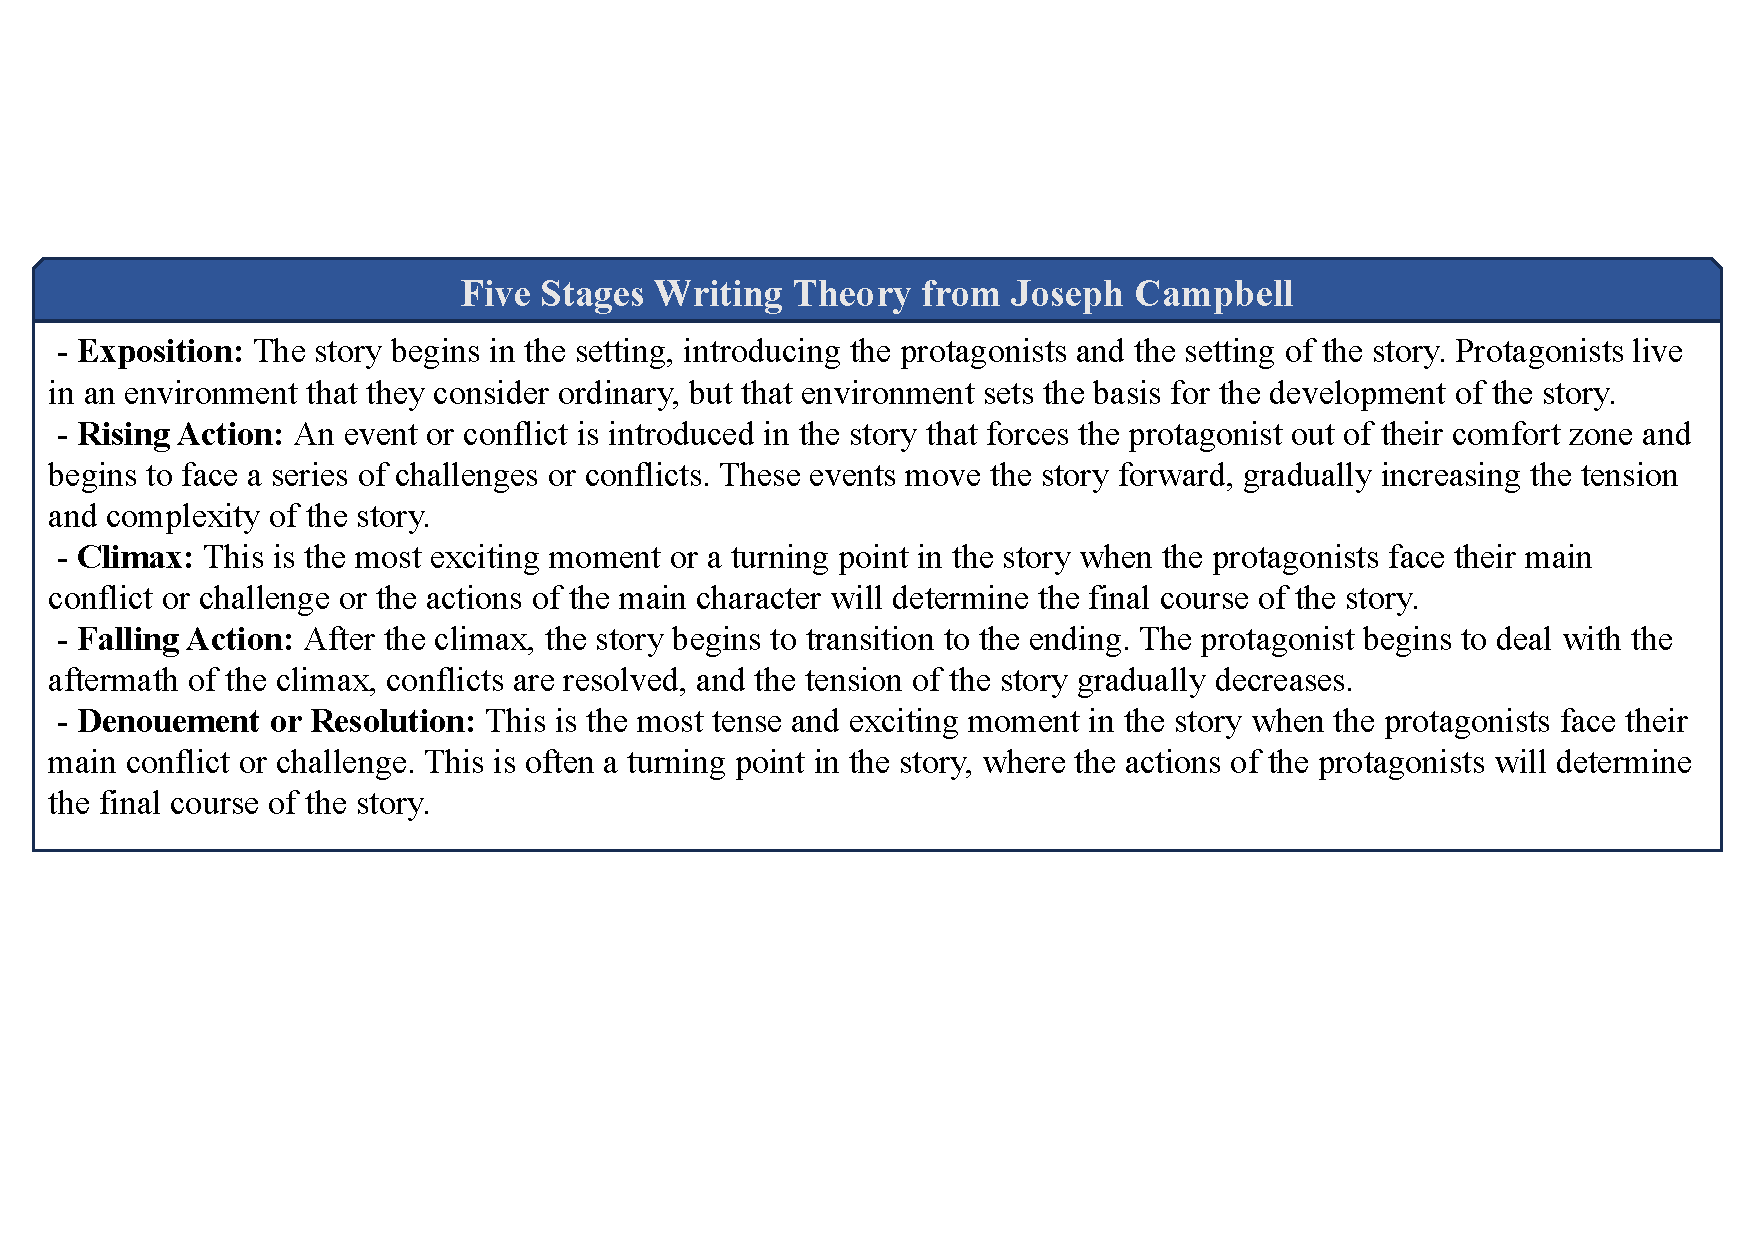
\includegraphics[width=0.95\linewidth]{images/novel_theory.pdf}

    \caption{\hjw{Five stages novel writing theory from Joseph Campbell \cite{TheoryFive}.}}  
    \label{fig:novel}
\vspace{-6pt}
\end{figure*}

\section{Problem definition and motivations}

\subsection{Problem Definition}

\wqyr{For a given story premise ${I}$ from a writer, we design a framework ${F^*}$ to generate a long-form story ${S}$. The score of story $S$ on the plot coherence is $C^{Plot}$ and the score of story $S$ on the context coherence is $C^{Context}$. We aim to generate a story ${S}$ with improved $C^{Plot}$ and $C^{Context}$.}


\subsection{Motivaiton}

\wqyr{Existing long-form story generation methods separate planning and writing stages based on the plan-write framework, making it impossible to adapt to the uncertainty of the writing stage. Besides, stories generated through this two-stage method tend to stop abruptly at the beginning, resulting in missing plots. Another method includes human-involved detail outline preferences, improving the flexibility of outlines but making the overall storyline uncontrollable or incomplete. An intuitive idea arises: \textit{What if we could further improve story coherence from plot fluency and completion?}}


\wqyr{The answer is yes. We follow the idea of the hierarchical outline \cite{DOC} which is composed of the rough outline and the detailed outline. To ensure the plot completeness, we consider the rough outline as the macro plot guidance and apply the novel writing theory to guide its generation to ensure it contains all the story stages of the theory. The detailed outlines are expanded gradually based on the corresponding rough outline referred to the relevant content in the leading story to improve the adaptability to the generation uncertainty. 
In addition, with the increasing length of the generated story, the contextual inconsistency becomes obvious \cite{Re3}. Therefore, we design a memory module to store stories and access concise relevant content. Since KG can model information and retrieve the relevant information ~\cite{pan2024unifying}, we apply KG to store and access the semantically relevant content with a filter based on LLM. By providing accurate and concise relevant content during the generation stage, this module can improve contextual consistency.}




